\documentclass[11pt,twocolumn]{article}
\usepackage[margin=0.72in]{geometry}
\usepackage{amsmath,amssymb,amsthm}
\usepackage{booktabs}
\usepackage{graphicx}
\usepackage{hyperref}
\usepackage{xcolor}
\usepackage{enumitem}

\hypersetup{
  colorlinks=true,
  linkcolor=blue!60!black,
  citecolor=green!45!black,
  urlcolor=blue!65!black
}

\newtheorem{theorem}{Theorem}
\newtheorem{definition}{Definition}

\newcommand{\ZZ}{\mathbb{Z}}
\newcommand{\QQ}{\mathbb{Q}}
\newcommand{\NN}{\mathbb{N}}

\title{\textbf{Machine-Checked Exact-Rational Dissimilarity, Binary-Counter, and Superpolynomial Space-Lower-Bound Certificates for Polynomial-Time Quantum Computation}}
\author{Lluis Eriksson\thanks{Independent researcher; manuscript prepared with transparent AI assistance via Google Antigravity. Source code, Lean~4 proofs, and exact certificates: \url{https://github.com/lluiseriksson/quantum-polytime-space-lower-bounds-certificates}.}}
\date{November 25, 2026}

\begin{document}
\maketitle

\begin{abstract}
A.\,C.\,Cem Say (\texttt{arXiv:2611.32633}, November 24, 2026) established unconditional space lower bounds for polynomial-time bounded-error quantum Turing machines (QTMs), proving that two-way quantum finite automata (2QCFAs) are strictly weaker than $o(\log\log n)$-space polynomial-time QTMs (Theorem~2, via $\ZZ^k$ word-problem dissimilarity) and uncovering an infinite hierarchy of languages $L_i$ separating sublogarithmic space classes $\Omega\!\bigl(\log n / (\log\log n)^i\bigr)$ (Theorem~3, via binary-counter two-track palindromes and a double-exponential runtime-vs.-space barrier). We present a machine-checked, zero-floating-point formalization and certificate auditing framework for the finite combinatorial, algebraic, and inequality core of these separations. First, we construct an 18-theorem zero-dependency Lean~4 kernel (\texttt{QuantumSpaceLowerBounds.lean}, Lean~4.35.0; 0~\texttt{sorry}, 0~warnings, 0~\texttt{Classical.choice}, 1 zero-axiom theorem) certifying arbitrary-dimension $\ZZ^k$ cancellation and dissimilarity ($\mathrm{Fin}\,k \to \ZZ$), unary binary-encoding length $\le (k+2)n$, exact 1D/2D/3D $L_1$-ball bounds, polynomial-degree domination $c\,n^u < n^k$, Remscrim's 2QCFA degree parameter $u = c(2r)^4 d^2 \ge 16$, $L_S$ binary-counter monotonicity, exact palindrome prefix separation on \texttt{List Bool} yielding $2^{j/2}$ dissimilar prefixes, Lemma~17 space-gap halving, and double-exponential vs.\ polynomial-degree dominance. Second, we define \texttt{QUANTUM-SPACE-LB-CERT-1.0} and a pure-stdlib zero-float verifier spanning four exact modes. Across 16 canonical certificates, replay runs in $0.013$--$4.440\,\mathrm{ms}$, passes direct brute-force $\ZZ^k$ $L_1$-ball, unary-injectivity, and $L_S$/$L_i$ cross-checks, and rejects 57/57 live adversarial forgeries.
\end{abstract}

\section{Introduction}
Unlike classical randomized space complexity—where Freivalds--Karpinski~\cite{freivalds1994space} and Dwork--Stockmeyer~\cite{dwork1990time} established sharp $\Omega(\log\log n)$ space lower bounds for nonregular languages—two-way quantum finite automata (2QCFAs) can recognize nonregular languages such as $\{a^n b^n\}$ and palindromes in polynomial or exponential time with $O(1)$ space~\cite{remscrim2020power}. Remscrim~\cite{remscrim2021lower} proved that any $r$-qubit, $d$-classical-state 2QCFA running in expected polynomial time on a language $L$ has dissimilarity function $D_L(n) = O(n^u)$ with $u = c(2r)^4 d^2$, and conjectured that polynomial-time sublogarithmic-space QTMs satisfy nontrivial lower bounds. Say~\cite{say2026quantumspace} resolved both frontiers: (i)~Theorem~2 constructs unary-encoded word problems $W_{\ZZ^k}$ whose dissimilarity grows as the $\ZZ^k$ $L_1$-ball $B_k(n) = \Omega(n^k)$, surpassing any fixed 2QCFA polynomial degree~$u$ for $k > u$; and (ii)~Theorem~3 builds two-track languages $L_i$ combining a binary-counter upper track $L_S$ with a lower-track palindrome of length $j_k = \Theta\!\bigl(\log N_k / (\log\log N_k)^i\bigr)$ ($2^{j_k/2}$ dissimilar prefixes), forcing superpolynomial runtime whenever QTM space falls in $o\!\bigl(\log n / (\log\log n)^i\bigr)$.

While the underlying quantum Markov-chain mixing and Remscrim spectral lower bounds~\cite{remscrim2021lower} are analytic, every finite combinatorial witness in~\cite{say2026quantumspace}—$\ZZ^k$ net-displacement dissimilarity, unary encoding lengths $\le (k+2)n$, exact polynomial-degree separation $c_k n^u < n^k$, $L_S$ populated lengths $N_k$, $L_i$ two-track palindromes, and Lemma~17's superpolynomial exponent gap $2^{\lfloor F \rfloor} - b_0 S > c L$—is purely exact over $\ZZ$ and $\QQ$. Floating-point approximations fail catastrophically on $n^k$ with $k = 2{,}049$ or $2^{31}$ vs.\ $100\cdot 2^{20}$; exact arbitrary-precision certification guarantees bit-exact verification.

\paragraph{Contributions.}
We formally verify and audit the finite combinatorial and algebraic backbone of~\cite{say2026quantumspace} (explicitly scoping our Lean~4 proofs away from the analytic spectral-gap and quantum Markov-chain simulation theorems of~\cite{remscrim2021lower,say2026quantumspace}):
\begin{enumerate}[leftmargin=*,nosep]
  \item \textbf{Zero-dependency Lean~4 kernel (\S\ref{sec:lean}):} 18 constructive theorems in \texttt{QuantumSpaceLowerBounds.lean} (Lean~4.35.0~\cite{demoura2021lean4}), 0~\texttt{sorry}, 0~warnings, 0~\texttt{Classical.choice}.
  \item \textbf{Exact-$\ZZ/\QQ$ verifier and schema (\S\ref{sec:certifier}):} \texttt{QUANTUM-SPACE-LB-CERT-1.0}, audited via Python's arbitrary-precision \texttt{int} and \texttt{fractions.Fraction} (zero floats) across four modes.
  \item \textbf{Empirical atlas, brute-force cross-checks, \& red-team audit (\S\ref{sec:results}):} 16 canonical certificates (full $\ZZ^k$ $L_1$-balls up to $k=4$, 2QCFA separation up to $k=2{,}049$, $L_i$ members for $i=0..3$, and Lemma~17 exponent barriers up to $L=2^{20}$) replayed in $0.013$--$4.440\,\mathrm{ms}$, brute-force cross-checks, and 57/57 rejected adversarial forgeries.
\end{enumerate}

\section{Combinatorial Structure of Say's Bounds}\label{sec:prelim}
\paragraph{Theorem~2 ($\ZZ^k$ word-problem separation).}
Let $W_{\ZZ^k}$ be the word problem of the free abelian group $\ZZ^k$ over generators $\{\pm g_1,\dots,\pm g_k\}$. Two words $w_1, w_2$ of length $\le n$ with distinct net displacements $u \neq v \in \ZZ^k$ are separated by $w_1^{-1}$, since $w_1 w_1^{-1} \in W_{\ZZ^k}$ while $w_2 w_1^{-1} \notin W_{\ZZ^k}$. Thus the dissimilarity count equals the exact $L_1$-ball cardinality
\begin{equation}
  B_k(n) = \bigl|\{x\!\in\!\ZZ^k : \|x\|_1\!\le\! n\}\bigr| = \!\sum_{j=0}^{\min(k,n)}\! 2^j \binom{k}{j}\binom{n}{j},
  \label{eq:ball}
\end{equation}
satisfying $B_1(n) = 2n+1$, $B_2(n) = 2n^2+2n+1$, and $3B_3(n) = 4n^3 + 6n^2 + 8n + 3$. Unary binary-alphabet encoding $\kappa_k$ maps each generator to at most $k+2$ bits ($|\kappa_k(w)| \le (k+2)n$). Since any $(r,d)$-2QCFA running in polynomial time obeys Remscrim's bound $D(n) = O(n^u)$ with $u = c(2r)^4 d^2$, choosing $k = u + 1$ yields $c_k n^u < n^k$ for all $n > c_k$.

\paragraph{Theorem~3 (Sublogarithmic hierarchy $L_i$).}
Define the binary counter string $u_k = \mathrm{bin}(0)\$\mathrm{bin}(1)\$\cdots\$\mathrm{bin}(k) \in L_S$ of length $N_k = |u_k|$, satisfying Say's Eq.~(4):
\begin{equation}
  2^L \le N_k \le 2^{2L}, \qquad L = |\mathrm{bin}(k)|, \quad M = |\mathrm{bin}(L)|.
  \label{eq:eq4}
\end{equation}
At hierarchy level $i \ge 0$, $L_i$ pairs upper track $u_k$ with a lower track $p\,\#^{N_k - j_k}$, where $p \in \{0,1\}^{j_k}$ is an even-length palindrome of length $j_k = 2^e$ ($e = \lceil L / M^i \rceil$ on finite witnesses, asymptotically $\Theta(L / M^i)$). Any two distinct left halves $\ell_1 \neq \ell_2 \in \{0,1\}^{j_k/2}$ are separated by suffix $\ell_1^R$, yielding $2^{j_k/2}$ dissimilar prefixes. Under a QTM using $S(n) \le a_0 X$ qubits ($X = L/M^i$) with Lemma~17 halving $2 b_0 a_0 \le d_2$, the exponent lower bound $F = (d_2 - b_0 a_0)X \ge \frac{d_2}{2} X$ satisfies the superpolynomial barrier
\begin{equation}
  2^{\lfloor F \rfloor} - b_0 S > c_{\mathrm{poly}}\,L,
  \label{eq:barrier}
\end{equation}
refuting $O(n^{c_{\mathrm{poly}}})$ runtime for every fixed polynomial degree~$c_{\mathrm{poly}}$.

\section{Zero-Dependency Lean 4 Kernel}\label{sec:lean}
We formalize 18 constructive theorems in \texttt{lean/QuantumSpaceLowerBounds.lean} (Lean~4.35.0, zero external libraries), audited via \texttt{lean/AuditAxioms.lean} with 0~warnings, 0~\texttt{sorry}, 0~\texttt{Classical.choice}, and 0~\texttt{Lean.ofReduceBool} (Table~\ref{tab:lean}).

\begin{theorem}[Constructive Quantum Space-LB Kernel]\label{thm:lean}
\leavevmode
\begin{enumerate}[leftmargin=*,nosep]
  \item \emph{Arbitrary-dimension $\ZZ^k$ dissimilarity \& 2QCFA separation:} Theorems~1--8 formalize coordinatewise cancellation $g + (-g) = 0$ and dissimilarity separation $u + (-u) = 0 \land v + (-u) \neq 0$ for arbitrary $k \in \NN$ over $\mathrm{Fin}\,k \to \ZZ$, unary encoding length $\le (k+2)n$, exact 1D/2D/3D $L_1$-ball bounds, strict polynomial-degree domination $c\,n^u < n^k$ ($k > u, n > c$), and Remscrim's $u = c(2r)^4 d^2 \ge 16$.
  \item \emph{Binary counter $L_S$ \& palindrome separation on \texttt{List Bool}:} Theorems~9--15 prove $|\mathrm{bin}(m)| \ge 1$, step gap $N_{k+1} - N_k = 1 + |\mathrm{bin}(k+1)| \ge 2$, strict monotonicity $a < b \implies N_a < N_b$, even palindrome length $2\cdot 2^{e-1} = 2^e$, $2^h \ge 2$, reverse involution $(p \mathbin{+\!\!+} p^R)^R = p \mathbin{+\!\!+} p^R$, and exact prefix separation ($\ell_1 \neq \ell_2$ of equal length implies $\ell_2 \mathbin{+\!\!+} \ell_1^R$ is not a palindrome).
  \item \emph{Lemma~17 halving \& superpolynomial dominance:} Theorems~16--18 prove cleared space-gap halving $2(d_2 X - b_0(a_0 X)) \ge d_2 X$, strict barrier subtraction $\mathrm{expF} - b_0 S > c L$, and inductive exponential dominance $2^m > m$ for all $m \in \NN$.
\end{enumerate}
\end{theorem}

\begin{table}[t]
\centering
\caption{Complete 18-theorem Lean~4.35.0 kernel in \texttt{QuantumSpaceLowerBounds.lean} (0~\texttt{sorry}, 0~warnings, 0~\texttt{Classical.choice}).}
\label{tab:lean}
\resizebox{\columnwidth}{!}{%
\begin{tabular}{@{}rll@{}}
\toprule
\# & Lean~4 Theorem Identifier & Axiom Footprint \\
\midrule
1 & \texttt{zk\_word\_problem\_cancel\_zero} & \texttt{[propext, Quot.sound]} \\
2 & \texttt{zk\_distinct\_displacement\_dissimilar} & \texttt{[propext, Quot.sound]} \\
3 & \texttt{zk\_unary\_encoding\_len\_bound} & \texttt{[propext, Quot.sound]} \\
4 & \texttt{zk\_ball\_1d\_exact} & \texttt{[propext, Quot.sound]} \\
5 & \texttt{zk\_ball\_2d\_exact} & \texttt{[propext, Quot.sound]} \\
6 & \texttt{zk\_ball\_3d\_exact\_cleared} & \texttt{[propext, Quot.sound]} \\
7 & \texttt{poly\_degree\_domination} & \texttt{[propext, Quot.sound]} \\
8 & \texttt{remscrim\_2qcfa\_exp\_u\_pos} & \texttt{[propext, Quot.sound]} \\
9 & \texttt{binary\_len\_pos} & \texttt{[propext, Quot.sound]} \\
10 & \texttt{binary\_counter\_step\_gap} & \texttt{[propext, Quot.sound]} \\
11 & \texttt{binary\_counter\_monotone\_len} & \texttt{[propext, Quot.sound]} \\
12 & \texttt{palindrome\_prefix\_half\_even} & \texttt{[propext, Quot.sound]} \\
13 & \texttt{palindrome\_dissimilarity\_exact\_pow2} & \texttt{none} \\
14 & \texttt{palindrome\_reverse\_involution} & \texttt{[propext]} \\
15 & \texttt{distinct\_left\_halves\_separated} & \texttt{[propext]} \\
16 & \texttt{space\_gap\_halving\_positive} & \texttt{[propext, Quot.sound]} \\
17 & \texttt{double\_exp\_beats\_poly\_exponent} & \texttt{[propext, Quot.sound]} \\
18 & \texttt{superpoly\_pow2\_dominates\_linear} & \texttt{[propext, Quot.sound]} \\
\bottomrule
\end{tabular}}
\end{table}

\section{Exact-Rational Certificate Architecture}\label{sec:certifier}
The pure-stdlib verifier \texttt{src/qspace\_certifier.py} audits \texttt{QUANTUM-SPACE-LB-CERT-1.0} certificates with zero floating-point arithmetic and strict JSON AST typing (rejecting \texttt{float}, \texttt{bool}, \texttt{Decimal}, \texttt{complex}, tuples, non-string keys, unreduced fractions, denominator-1 strings, and \texttt{"-0"}) across four exact modes:

\begin{definition}[Four \texttt{QUANTUM-SPACE-LB-CERT-1.0} Modes]\label{def:modes}
\leavevmode
\begin{enumerate}[leftmargin=*,nosep]
  \item \textbf{Mode~1} (\texttt{\small zk\_\allowbreak word\_\allowbreak problem\_\allowbreak dissimilarity\_\allowbreak exact}): Audits a set of words over $\{\pm 1,\dots,\pm k\}$ of length $\le n$, verifying pairwise distinct $\ZZ^k$ net displacements, explicit separating suffixes $w_i^{-1}$, unary binary-encoding bound $|\kappa_k(w)| \le (k+2)n$, exact $B_k(n)$~\eqref{eq:ball}, and max encoded length.
  \item \textbf{Mode~2} (\texttt{\small poly\_\allowbreak degree\_\allowbreak 2qcfa\_\allowbreak separation\_\allowbreak exact}): Audits Remscrim's exact 2QCFA degree $u = c(2r)^4 d^2$, separating dimension $k > u$, and arbitrary-precision inequality $c_k n^u < n^k$ (up to $k=2{,}049, n=512$).
  \item \textbf{Mode~3} (\texttt{\small sublog\_\allowbreak hierarchy\_\allowbreak Li\_\allowbreak membership\_\allowbreak exact}): Audits two-track membership in $L_i$: exact upper-track binary counter $u_k \in L_S$, Eq.~\eqref{eq:eq4} bounds $2^L \le N_k \le 2^{2L}$, exact lower-track palindrome $p \in \{0,1\}^{j_k}$ with $p = p^R$, padding $\#^{N_k - j_k}$, and $\log_2$-dissimilarity $j_k/2$.
  \item \textbf{Mode~4} (\texttt{\small sublog\_\allowbreak space\_\allowbreak exponent\_\allowbreak barrier\_\allowbreak exact}): Audits exact bit-length $2^{M-1} \le L < 2^M$, Lemma~17 halving $2 b_0 a_0 \le d_2$, exact rational lower bound $F_{\mathrm{lb}} = (d_2 - b_0 a_0) L / M^i$, and superpolynomial barrier~\eqref{eq:barrier} $2^{\lfloor F_{\mathrm{lb}}\rfloor} - b_0 S > c_{\mathrm{poly}} L$.
\end{enumerate}
\end{definition}

\section{Empirical Atlas and Red-Team Verification}\label{sec:results}
All 16 canonical certificates and four experiment logs are generated deterministically by \texttt{scripts/run\_all\_experiments.py} and audited end-to-end by \texttt{scripts/verify\_all.py} (Lean~4 build, 18/18 axiom audit, 16/16 cert replay, \texttt{pytest}, and 39/39 SHA-256 hashes).

\paragraph{1. Exact $\ZZ^k$ dissimilarity growth and 2QCFA degree separation.}
Figure~\ref{fig:zk-2qcfa}(a) plots exact $L_1$-ball dissimilarity $B_k(n)$~\eqref{eq:ball} across $k \in \{1,\dots,5\}$ and $n \in \{1,\dots,12\}$: at $n=12$, $B_k(12)$ climbs from $25$ ($k=1$) and $313$ ($k=2$) through $2{,}625$ ($k=3$) and $16{,}641$ ($k=4$) to $85{,}305$ ($k=5$). Figure~\ref{fig:zk-2qcfa}(b) contrasts Remscrim's 2QCFA upper degree $u = c(2r)^4 d^2$ against the minimal separating lattice dimension $k = u + 1$ across four configurations, culminating in $(c=2, r=2, d=2) \implies u = 2{,}048, k = 2{,}049$, where exact integer comparison verifies $c_k n^{2048} < n^{2049}$ at $n=512$ in $0.105\,\mathrm{ms}$.

\begin{figure}[t]
\centering
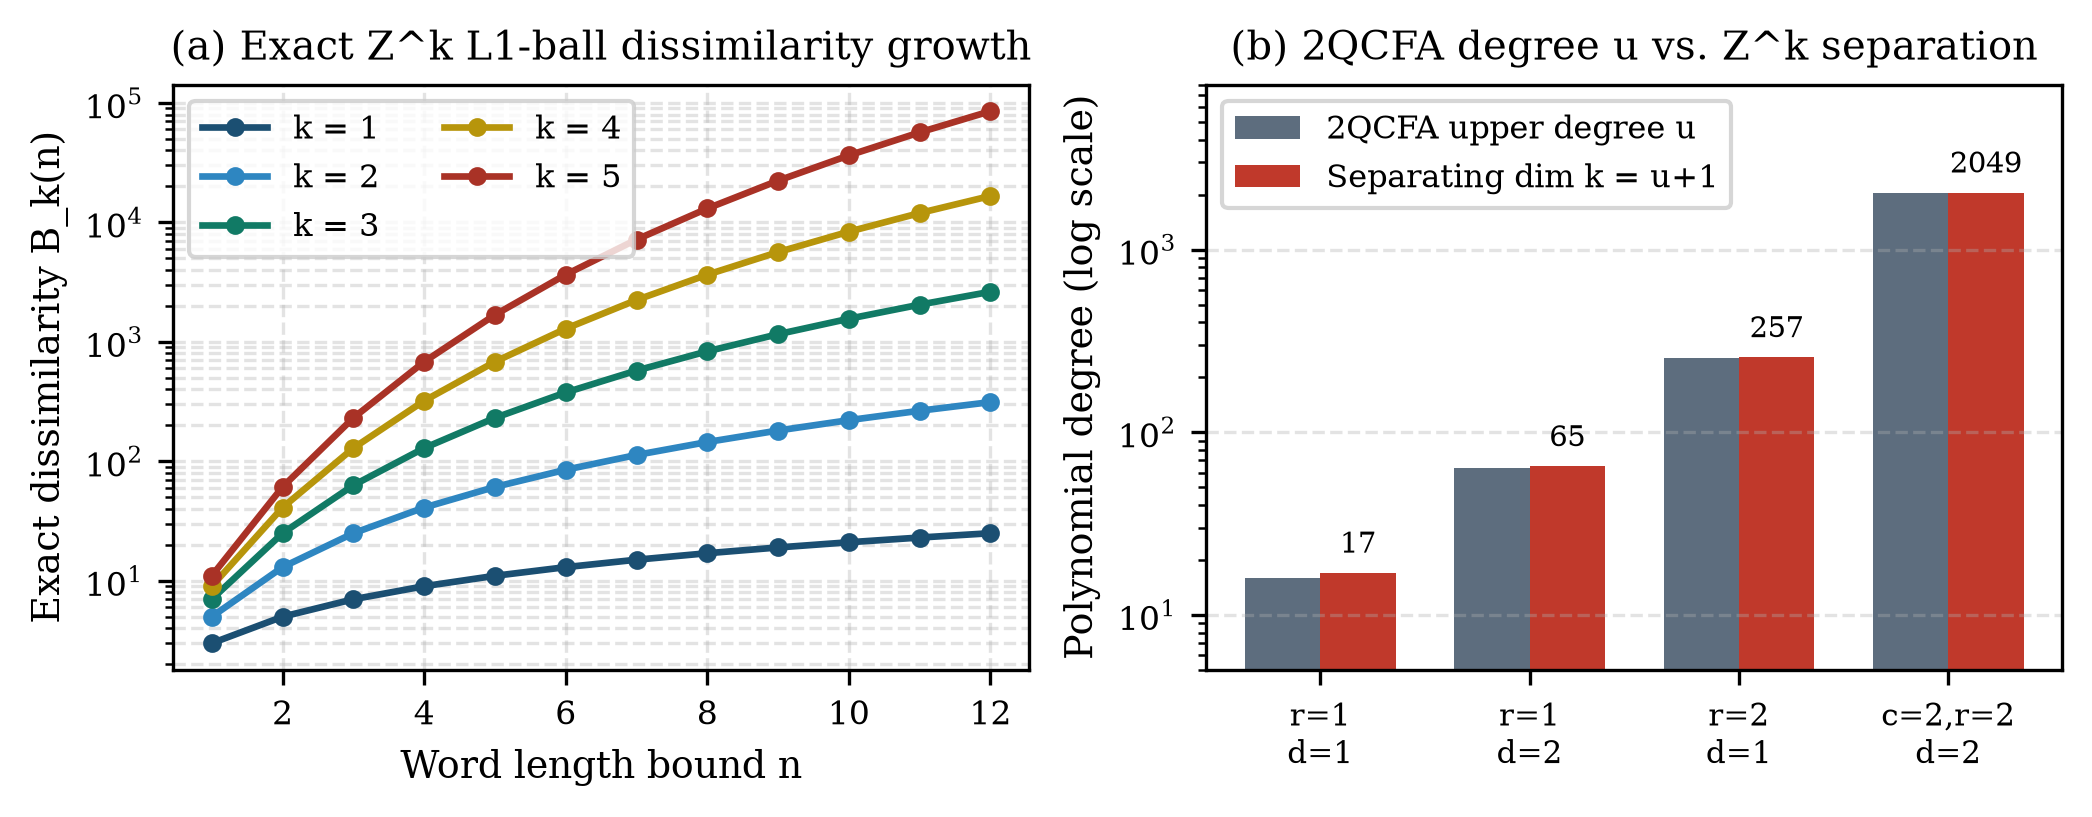
\includegraphics[width=\columnwidth]{figures/fig1_zk_ball_and_2qcfa.png}
\caption{(a)~Exact $\ZZ^k$ $L_1$-ball dissimilarity $B_k(n)$ for $k=1..5, n=1..12$. (b)~Remscrim 2QCFA polynomial degree $u = c(2r)^4 d^2$ versus minimal separating dimension $k = u + 1$.}
\label{fig:zk-2qcfa}
\end{figure}

\paragraph{2. Binary-counter $L_S$ scaling and sublogarithmic hierarchy $L_i$.}
Figure~\ref{fig:counter-sublog}(a) tracks exact $L_S$ counter lengths $N_k$ ($25, 65, 161, 385, 897, 2{,}049$ for $k = 2^b - 1$, $b=3..8$) alongside finite-scale palindrome prefix lengths $j_k$ for $i=0,1,2$ (where $j_k$ at $i=1$ exhibits the discrete ceiling step $L=7, M=3 \implies \lceil 7/3 \rceil = 3$ to $L=8, M=4 \implies \lceil 8/4 \rceil = 2$ as $|\mathrm{bin}(L)|$ increments). Figure~\ref{fig:counter-sublog}(b) traces the smooth sublogarithmic space-threshold hierarchy $L / M^i$ ($i=0..3$) across $L \in [2^4, 2^{15}]$, showing the clean polylogarithmic separation between consecutive levels of Theorem~3.

\begin{figure}[t]
\centering
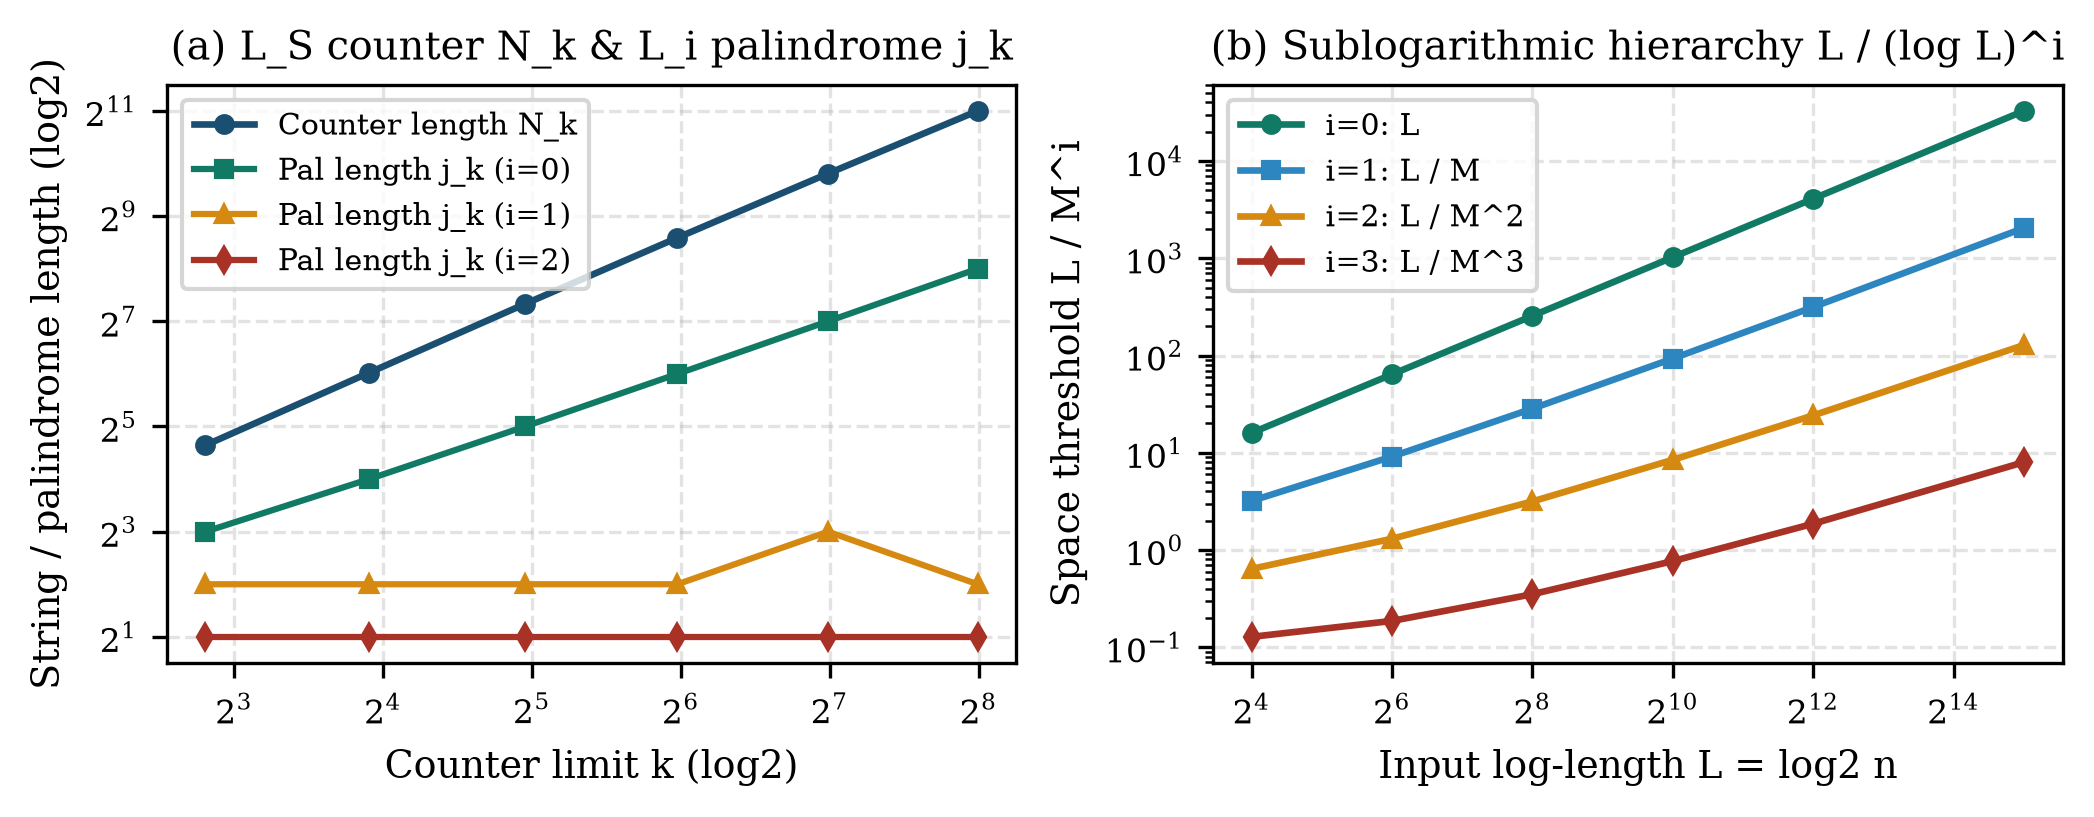
\includegraphics[width=\columnwidth]{figures/fig2_counter_and_sublog_hierarchy.png}
\caption{(a)~Exact $L_S$ counter lengths $N_k$ and $L_i$ palindrome prefix lengths $j_k$ for $k \in \{7,\dots,255\}$. (b)~Sublogarithmic hierarchy space thresholds $L / M^i$ across $L \in [16, 32768]$ for $i=0..3$.}
\label{fig:counter-sublog}
\end{figure}

\paragraph{3. 16-certificate atlas, brute-force cross-checks, and 57-attack suite.}
Table~\ref{tab:atlas} and Figure~\ref{fig:atlas} summarize all 16 canonical certificates, replayed with zero floats in $0.013$--$4.440\,\mathrm{ms}$ (including full $L_1$-ball witnesses of sizes $13, 41, 63, 129$ in Mode~1 and $L = 2^{20}$ exponent barrier $2^{31} \gg 100\cdot 2^{20}$ in Mode~4). In \texttt{tests/test\_suite.py}, independent tests cross-check $B_k(n)$ by brute-force integer-lattice enumeration across $k=1..4$, verify Eq.~\eqref{eq:eq4} and monotonicity of $N_k$ across $k=4..128$, verify unary encoding injectivity on all length-$\le 2$ words in $\ZZ^3$, replay all 16 certificates, and confirm 57/57 live adversarial forgeries (commuting-word collisions, generator overflow, $k=u$, non-palindrome lower tracks, Eq.~\eqref{eq:eq4}/bit-length mismatches, violated halving $2b_0 a_0 > d_2$, and breached exponent barriers) are rejected with \texttt{QuantumSpaceLBCertificateError}.

\begin{figure}[t]
\centering
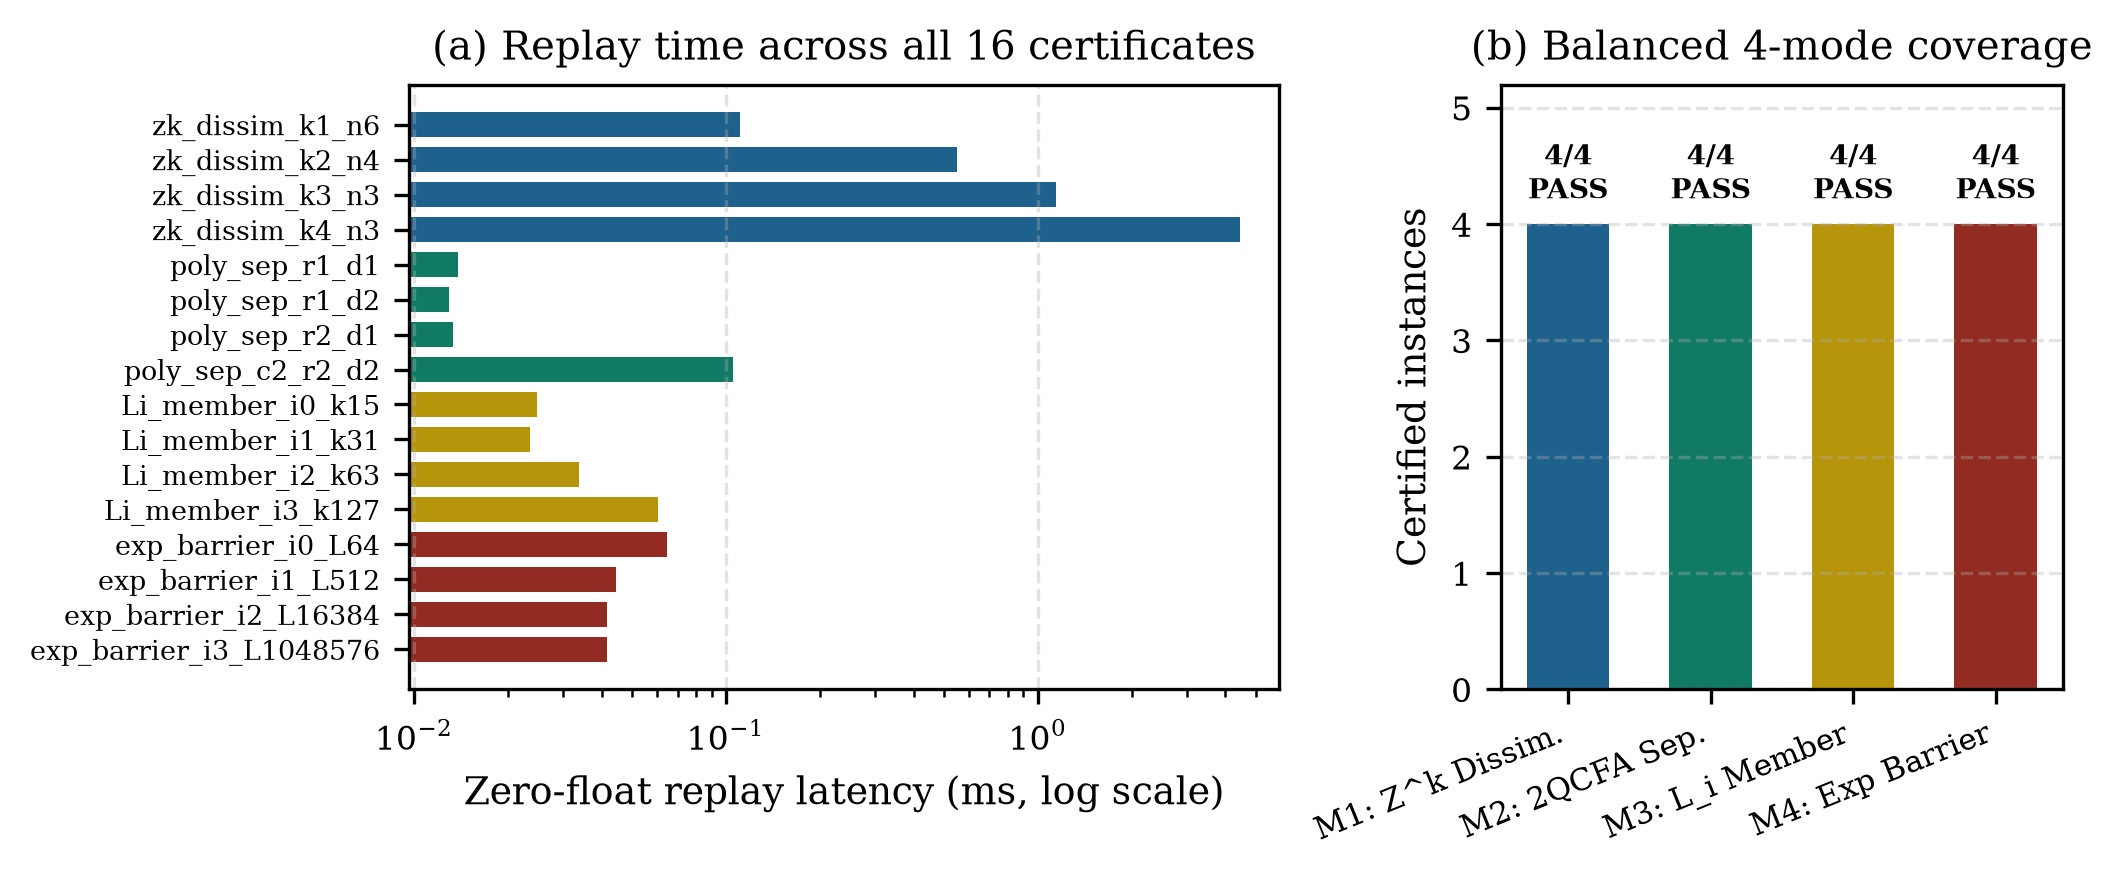
\includegraphics[width=\columnwidth]{figures/fig3_atlas_summary.png}
\caption{(a)~Zero-float replay latency across all 16 canonical \texttt{QUANTUM-SPACE-LB-CERT-1.0} certificates ($0.013$--$4.440\,\mathrm{ms}$, log scale). (b)~Balanced 4-per-mode coverage across all four verification modes.}
\label{fig:atlas}
\end{figure}

\begin{table}[t]
\centering
\caption{Summary of all 16 exact-$\ZZ/\QQ$ \texttt{QUANTUM-SPACE-LB-CERT-1.0} certificates (zero floating-point arithmetic; reference-machine replay latency in ms).}
\label{tab:atlas}
\resizebox{\columnwidth}{!}{%
\begin{tabular}{@{}lllr@{}}
\toprule
Certificate File (stem) & Mode & Key Exact Witness & ms \\
\midrule
\texttt{zk\_dissim\_k1\_n6} & M1 & $k=1, n=6$: $13/13$ ball, enc $\le 18$ & 0.111 \\
\texttt{zk\_dissim\_k2\_n4} & M1 & $k=2, n=4$: $41/41$ ball, enc $\le 16$ & 0.550 \\
\texttt{zk\_dissim\_k3\_n3} & M1 & $k=3, n=3$: $63/63$ ball, enc $\le 15$ & 1.144 \\
\texttt{zk\_dissim\_k4\_n3} & M1 & $k=4, n=3$: $129/129$ ball, enc $\le 18$ & 4.440 \\
\texttt{poly\_sep\_r1\_d1} & M2 & $u=16, k=17, n=64$ & 0.014 \\
\texttt{poly\_sep\_r1\_d2} & M2 & $u=64, k=65, n=128$ & 0.013 \\
\texttt{poly\_sep\_r2\_d1} & M2 & $u=256, k=257, n=256$ & 0.013 \\
\texttt{poly\_sep\_c2\_r2\_d2} & M2 & $u=2048, k=2049, n=512$ & 0.105 \\
\texttt{Li\_member\_i0\_k15} & M3 & $i=0, k=15$: $N_k=65, j_k=16$ & 0.025 \\
\texttt{Li\_member\_i1\_k31} & M3 & $i=1, k=31$: $N_k=161, j_k=4$ & 0.024 \\
\texttt{Li\_member\_i2\_k63} & M3 & $i=2, k=63$: $N_k=385, j_k=2$ & 0.034 \\
\texttt{Li\_member\_i3\_k127} & M3 & $i=3, k=127$: $N_k=897, j_k=2$ & 0.060 \\
\texttt{exp\_barrier\_i0\_L64} & M4 & $i=0, L=64$: $\lfloor F\rfloor=13, c=10$ & 0.065 \\
\texttt{exp\_barrier\_i1\_L512} & M4 & $i=1, L=512$: $\lfloor F\rfloor=14, c=20$ & 0.044 \\
\texttt{exp\_barrier\_i2\_L16384} & M4 & $i=2, L=2^{14}$: $\lfloor F\rfloor=20, c=50$ & 0.042 \\
\texttt{exp\_barrier\_i3\_L1048576} & M4 & $i=3, L=2^{20}$: $\lfloor F\rfloor=31, c=100$ & 0.042 \\
\bottomrule
\end{tabular}}
\end{table}

\section{Scope, Limitations, and Conclusion}\label{sec:conclusion}
This work machine-checks the finite combinatorial, dissimilarity-growth, binary-counter, and superpolynomial exponent-separation core of Say's polynomial-time quantum space lower bounds~\cite{say2026quantumspace}, and delivers a zero-float exact-$\ZZ/\QQ$ certificate auditor spanning $\ZZ^k$ $L_1$-balls, Remscrim 2QCFA degree separation, two-track $L_i$ witnesses, and Lemma~17 exponent barriers. It does \emph{not} formalize the analytic quantum Markov-chain spectral theory of Remscrim~\cite{remscrim2021lower} or the full QTM simulation reductions of~\cite{say2026quantumspace} in Lean~4. Within its verified scope, the Lean~4 kernel and \texttt{QUANTUM-SPACE-LB-CERT-1.0} auditor provide exact, manifest-locked verification for sublogarithmic quantum space separations.

\bibliographystyle{plain}
\bibliography{references}
\end{document}
